\documentclass[12pt]{article}
\usepackage[a4paper,margin=1in]{geometry}
\usepackage{graphicx}
\usepackage{amsmath}
\usepackage{hyperref}
\usepackage[outputdir=../]{minted}
% for the above code thank the increadble StackExchange forum https://tex.stackexchange.com/questions/531738/minted-environment-not-working-in-overleaf

\begin{document}

%-------------------- Title Page --------------------
\title{Laboratory 1: Circuit Designs and Testing}
\author{Shein Htike \and Brandon Vasquez}
\date{CSC 343 Spring 2025}
\maketitle

\tableofcontents
\clearpage

\section{Exercise A: 8x1 Multiplexer Using Logic Gates}
\subsection{Objective}
The goal of this exercise is to create an 8x1 multiplexer in two ways: using logic gates and using VHDL code.
\subsection{Functionality and Specifications}
\subsubsection{Logic}
The output of the 8×1 multiplexer is given by the following logic equation:

\begin{equation}
\begin{split}
\text{output} =\,& \overline{S_2}\,\overline{S_1}\,\overline{S_0}\,I_0 \ \vee\ \overline{S_2}\,\overline{S_1}\,S_0\,I_1 \ \vee \\[1mm]
                & \overline{S_2}\,S_1\,\overline{S_0}\,I_2 \ \vee\ \overline{S_2}\,S_1\,S_0\,I_3 \ \vee \\[1mm]
                & S_2\,\overline{S_1}\,\overline{S_0}\,I_4 \ \vee\ S_2\,\overline{S_1}\,S_0\,I_5 \ \vee \\[1mm]
                & S_2\,S_1\,\overline{S_0}\,I_6 \ \vee\ S_2\,S_1\,S_0\,I_7 
\end{split}
\end{equation}

In this multiplexer design, we select one of the eight inputs, $I_{0}$ through $I_{7}$ and connect it to a single output based on the binary value of the three select signals, $S_{2}$, $S_{1}$, and $S_{0}$ (with $S_{2}$ being the most significant bit).
\clearpage
\subsubsection{Circut Design}
In order to implement the 8x1 multiplexer, we created this circuit design in Intel Quartus Prime.
This circuit was then compiled into VHDL and imported into ModelSim in order to simulate and test our design. \\

\subsection{Functionality and Specifications}
\begin{figure}[h]
\caption{8x1 multiplexer}
\centering
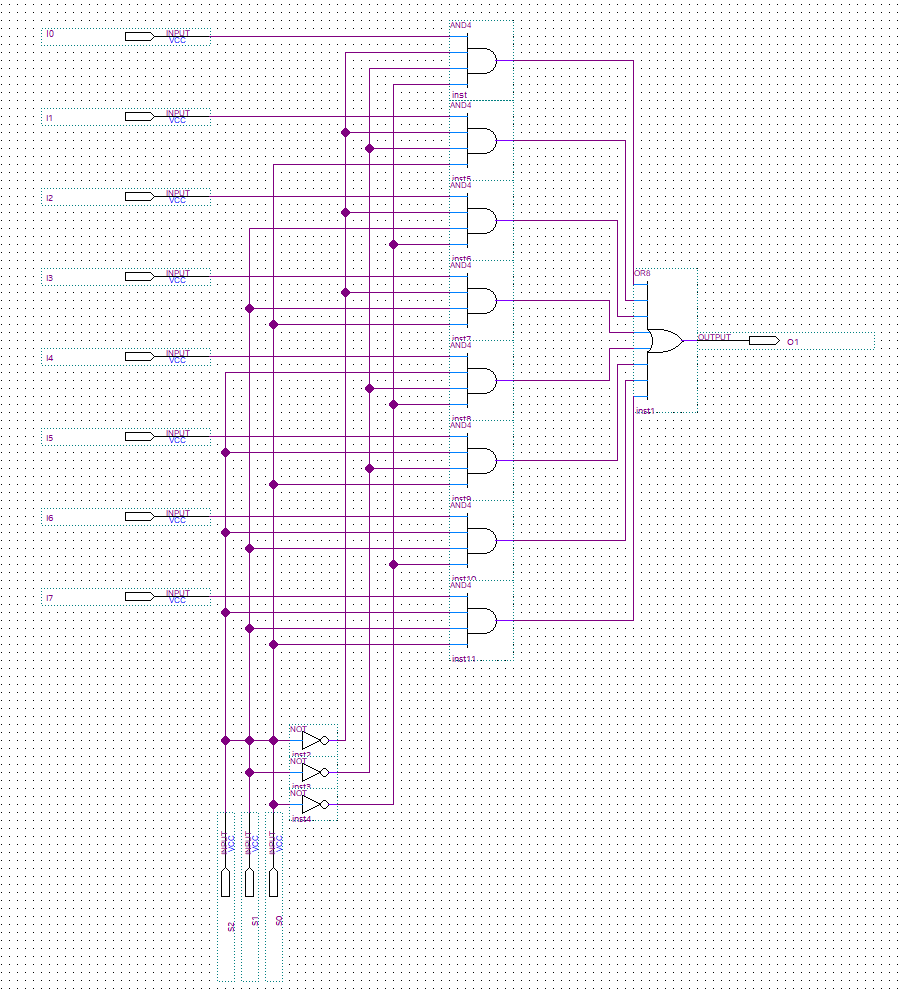
\includegraphics[width=\textwidth]{./diagrams/8x1multiplexer.png}
\end{figure}

\clearpage
\subsubsection{VHDL Code}
I also redesigned this multiplexer in VHDL using behavioral modeling.
\begin{minted}[linenos]{vhdl}
    library IEEE;
    use IEEE.std_logic_1164.all;
    
    entity multiplexer8x1v2 is
        port (
            I : in  std_logic_vector(7 downto 0);
            S : in  std_logic_vector(2 downto 0);
            O : out std_logic
        );
    end multiplexer8x1v2;
    
    architecture Behavioral of multiplexer8x1v2 is
    begin
        with S select
            O <= I(0) when "000",
                 I(1) when "001",
                 I(2) when "010",
                 I(3) when "011",
                 I(4) when "100",
                 I(5) when "101",
                 I(6) when "110",
                 I(7) when "111",
                 '0'    when others;  -- Default case if needed
    end Behavioral;
\end{minted}
\clearpage

\subsection{Simulation}
I wrote VHDL to simulate both versions of the circuit.
\subsubsection{Structural Model Test Bench}

\begin{minted}{vhdl}
LIBRARY IEEE;
USE IEEE.STD_LOGIC_1164.ALL;
USE IEEE.STD_LOGIC_TEXTIO.ALL;
USE std.textio.ALL;

ENTITY tb_multiplexer8x1 IS
END tb_multiplexer8x1;

ARCHITECTURE test OF tb_multiplexer8x1 IS
    SIGNAL I0 : STD_LOGIC := '0';
    SIGNAL I1 : STD_LOGIC := '0';
    SIGNAL I2 : STD_LOGIC := '0';
    SIGNAL I3 : STD_LOGIC := '0';
    SIGNAL I4 : STD_LOGIC := '0';
    SIGNAL I5 : STD_LOGIC := '0';
    SIGNAL I6 : STD_LOGIC := '0';
    SIGNAL I7 : STD_LOGIC := '0';
    SIGNAL S2 : STD_LOGIC := '0';
    SIGNAL S1 : STD_LOGIC := '0';
    SIGNAL S0 : STD_LOGIC := '0';
    SIGNAL O1 : STD_LOGIC;

    COMPONENT mux8to1_structural IS
        PORT (
            I0 : IN STD_LOGIC;
            I2 : IN STD_LOGIC;
            I3 : IN STD_LOGIC;
            I1 : IN STD_LOGIC;
            I4 : IN STD_LOGIC;
            I5 : IN STD_LOGIC;
            I6 : IN STD_LOGIC;
            I7 : IN STD_LOGIC;
            S2 : IN STD_LOGIC;
            S1 : IN STD_LOGIC;
            S0 : IN STD_LOGIC;
            O1 : OUT STD_LOGIC
        );
    END COMPONENT;

BEGIN
    uut : mux8to1_structural
    PORT MAP(I0, I2, I3, I1, I4, I5, I6, I7, S2, S1, S0, O1);

    PROCESS
    BEGIN
        S2 <= '0';
        S1 <= '0';
        S0 <= '0';
        WAIT FOR 10 ns;
        I0 <= '1';
        WAIT FOR 10 ns;
        I0 <= '0';

        S2 <= '0';
        S1 <= '0';
        S0 <= '1';
        WAIT FOR 10 ns;
        I1 <= '1';
        WAIT FOR 10 ns;
        I1 <= '0';

        S2 <= '0';
        S1 <= '1';
        S0 <= '0';
        WAIT FOR 10 ns;
        I2 <= '1';
        WAIT FOR 10 ns;
        I2 <= '0';

        S2 <= '0';
        S1 <= '1';
        S0 <= '1';
        WAIT FOR 10 ns;
        I3 <= '1';
        WAIT FOR 10 ns;
        I3 <= '0';

        S2 <= '1';
        S1 <= '0';
        S0 <= '0';
        WAIT FOR 10 ns;
        I4 <= '1';
        WAIT FOR 10 ns;
        I4 <= '0';

        S2 <= '1';
        S1 <= '0';
        S0 <= '1';
        WAIT FOR 10 ns;
        I5 <= '1';
        WAIT FOR 10 ns;
        I5 <= '0';

        S2 <= '1';
        S1 <= '1';
        S0 <= '0';
        WAIT FOR 10 ns;
        I6 <= '1';
        WAIT FOR 10 ns;
        I6 <= '0';

        S2 <= '1';
        S1 <= '1';
        S0 <= '1';
        WAIT FOR 10 ns;
        I7 <= '1';
        WAIT FOR 10 ns;
        I7 <= '0';
    END PROCESS;
END test;

\end{minted}
This code selects inputs 0 through 7 and toggles them while they are selected to show that the output corresponds to the selected input.

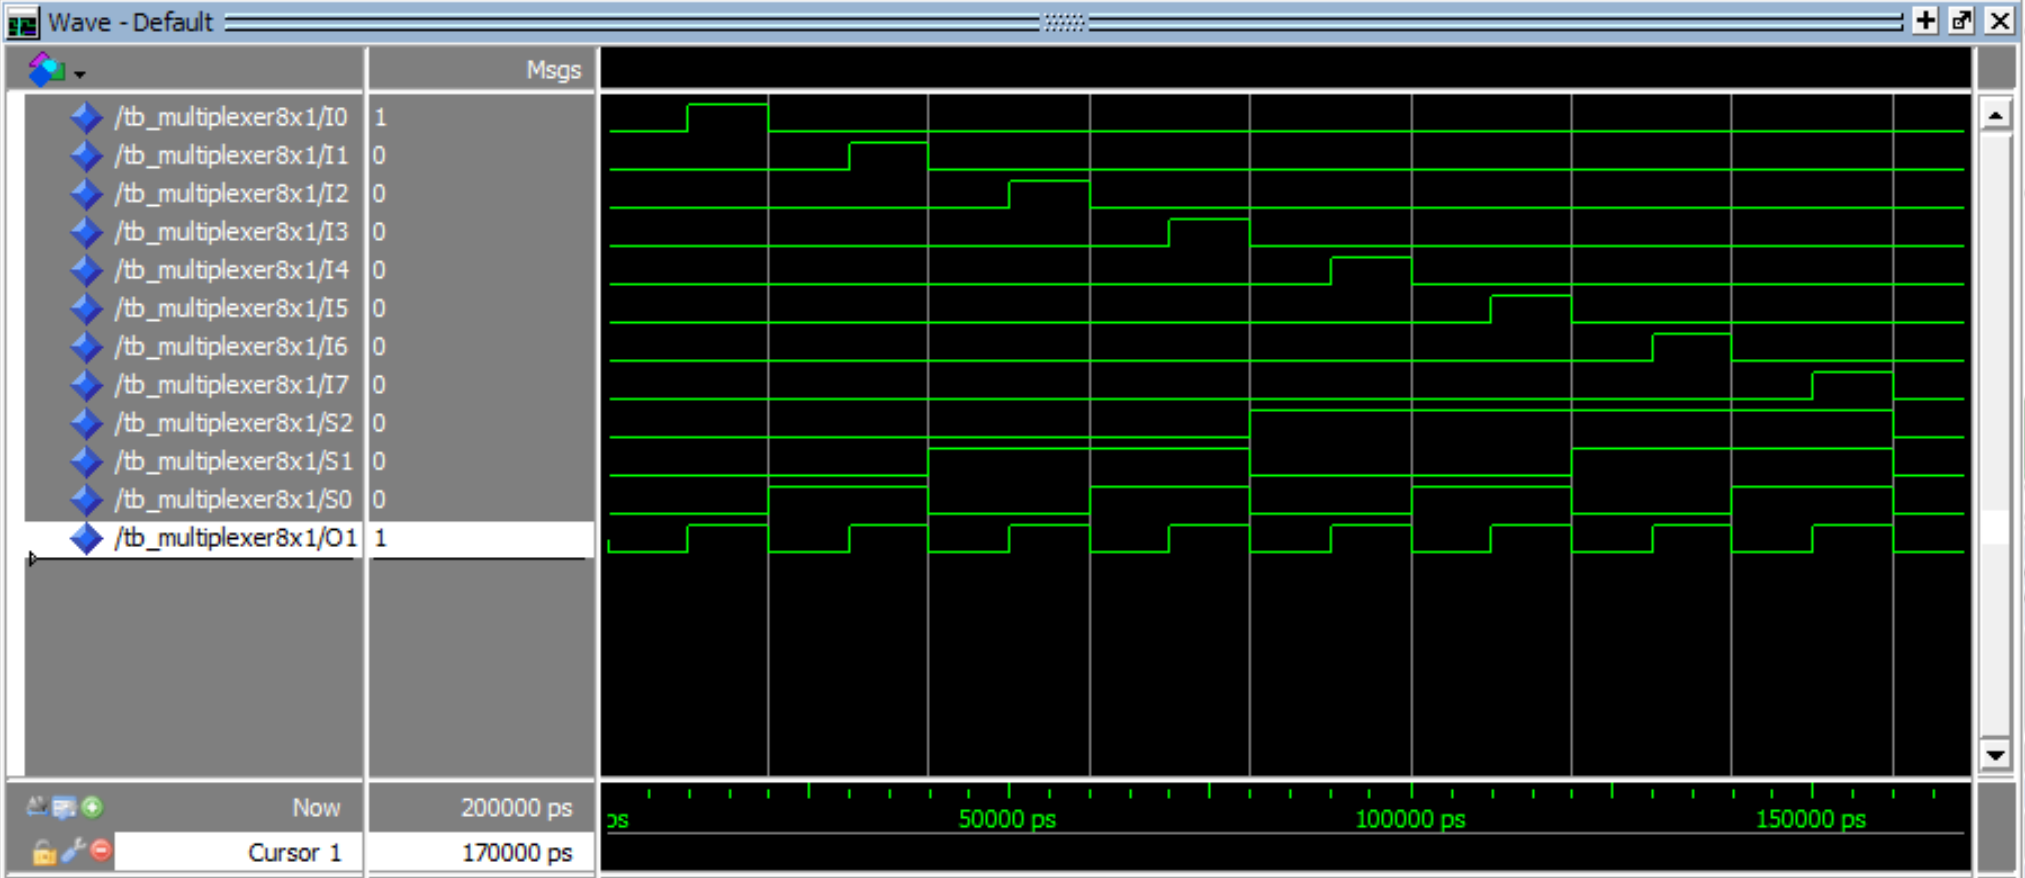
\includegraphics[width=\textwidth]{mux_structural.png}
\clearpage
\subsubsection{Behavioral Model Test Bench}
I also wrote test bench code for the behavioral model multiplexer. This code was essentially the same as the previous test bench for the structural model. The only difference is that the inputs and the select signals were vectors.
\begin{minted}{vhdl}
    LIBRARY IEEE;
USE IEEE.STD_LOGIC_1164.ALL;
USE IEEE.STD_LOGIC_TEXTIO.ALL;
USE STD.TEXTIO.ALL;

ENTITY tb_multiplexer8x1v2 IS
END tb_multiplexer8x1v2;

ARCHITECTURE test OF tb_multiplexer8x1v2 IS
    SIGNAL I : STD_LOGIC_VECTOR(7 DOWNTO 0) := (OTHERS => '0');
    SIGNAL S : STD_LOGIC_VECTOR(2 DOWNTO 0) := "000";
    SIGNAL O : STD_LOGIC;
    COMPONENT multiplexer8x1v2 IS
        PORT (
            I : IN  STD_LOGIC_VECTOR(7 DOWNTO 0);
            S : IN  STD_LOGIC_VECTOR(2 DOWNTO 0);
            O : OUT STD_LOGIC
        );
    END COMPONENT;
BEGIN
    uut : multiplexer8x1v2
        PORT MAP (
            I => I,
            S => S,
            O => O
        );
    PROCESS
    BEGIN
        S <= "000";
        I <= (OTHERS => '0');
        WAIT FOR 10 ns;
        I(0) <= '1';
        WAIT FOR 10 ns;
        I(0) <= '0';
        S <= "001";
        I <= (OTHERS => '0');
        WAIT FOR 10 ns;
        I(1) <= '1';
        WAIT FOR 10 ns;
        I(1) <= '0';
        S <= "010";
        I <= (OTHERS => '0');
        WAIT FOR 10 ns;
        I(2) <= '1';
        WAIT FOR 10 ns;
        I(2) <= '0';
        S <= "011";
        I <= (OTHERS => '0');
        WAIT FOR 10 ns;
        I(3) <= '1';
        WAIT FOR 10 ns;
        I(3) <= '0';
        S <= "100";
        I <= (OTHERS => '0');
        WAIT FOR 10 ns;
        I(4) <= '1';
        WAIT FOR 10 ns;
        I(4) <= '0';
        S <= "101";
        I <= (OTHERS => '0');
        WAIT FOR 10 ns;
        I(5) <= '1';
        WAIT FOR 10 ns;
        I(5) <= '0';
        S <= "110";
        I <= (OTHERS => '0');
        WAIT FOR 10 ns;
        I(6) <= '1';
        WAIT FOR 10 ns;
        I(6) <= '0';
        S <= "111";
        I <= (OTHERS => '0');
        WAIT FOR 10 ns;
        I(7) <= '1';
        WAIT FOR 10 ns;
        I(7) <= '0';
        WAIT;
    END PROCESS;
END test;
\end{minted}
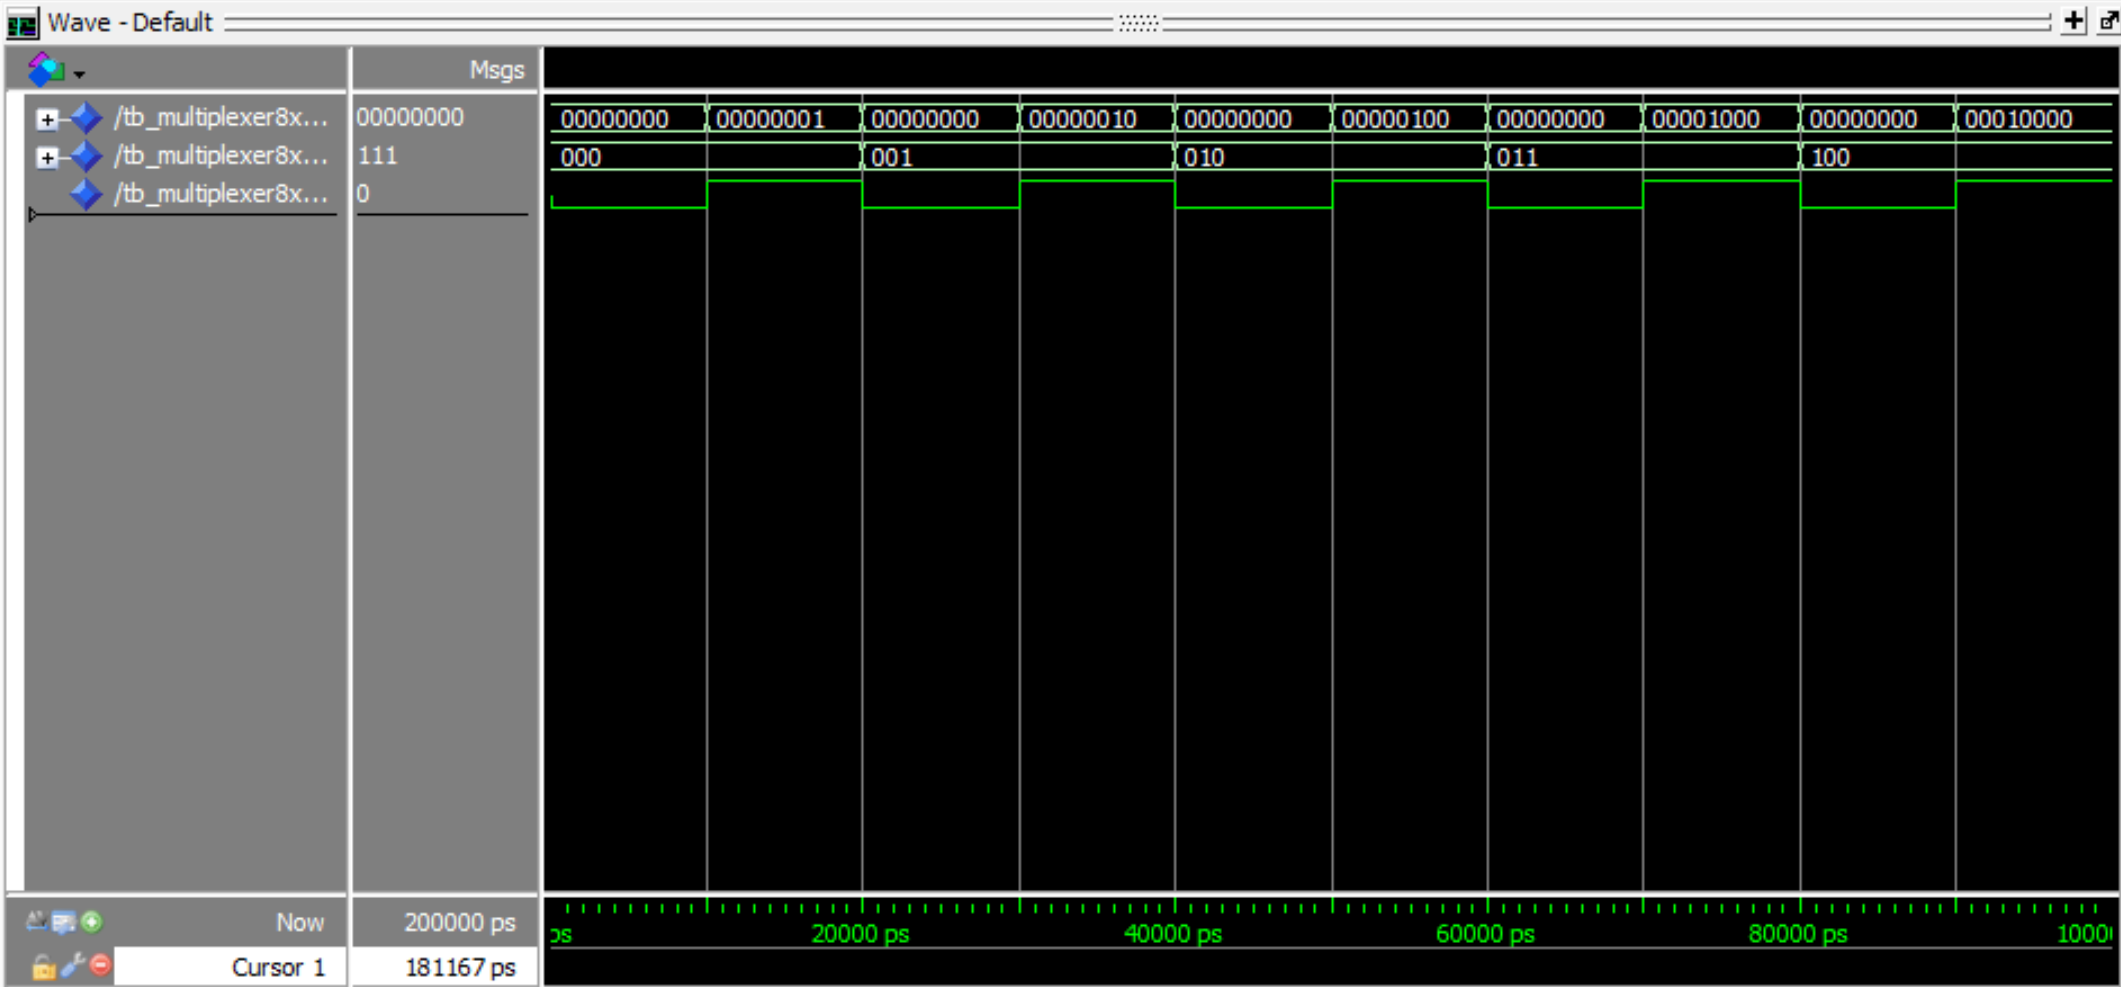
\includegraphics[width=\textwidth]{mux_behavioral.png}
\clearpage


\section{Exercise B: 1x8 De-Multiplexer Using 1x4 and 1x2 De-Multiplexers}
\subsection{Objective}

\subsection{Functionality and Specifications}

\subsection{Simulation}
\clearpage
%-------------------- 3x8 decoder begin --------------------
\section{Exercise C: 3-to-8 Decoder}
\subsection{Objective}
The purpose of this exercise was to create a 3x8 decoder circuit from its respective combinational logic. Now having compiled and generated the relevant VHDL for the circuit one was able to simulate the circuit in action.

\subsection{Functionality and Specifications}

Here we want to describe the combinational logic functions (Boolean equations, if applicable)

\begin{figure}[h]
\caption{3x8 decoder}
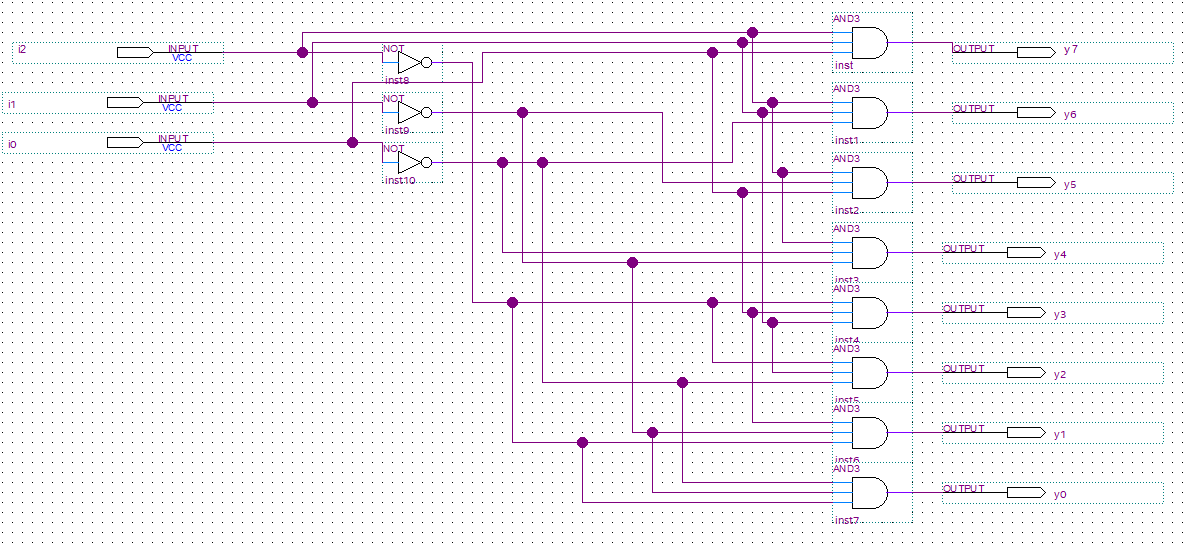
\includegraphics[width=\textwidth]{./diagrams/3x8_decoder.png}
\end{figure}
\subsubsection{VHDL Code generated from the design file}
\begin{minted}{vhdl}
    LIBRARY ieee;
    USE ieee.std_logic_1164.all;

    LIBRARY work;

    ENTITY lab_assign_1 IS
    	PORT
    	(
    		i2 :  IN  STD_LOGIC;
    		i1 :  IN  STD_LOGIC;
    		i0 :  IN  STD_LOGIC;
    		y7 :  OUT  STD_LOGIC;
    		y6 :  OUT  STD_LOGIC;
    		y5 :  OUT  STD_LOGIC;
    		y4 :  OUT  STD_LOGIC;
    		y3 :  OUT  STD_LOGIC;
    		y2 :  OUT  STD_LOGIC;
    		y1 :  OUT  STD_LOGIC;
    		y0 :  OUT  STD_LOGIC
    	);
    END lab_assign_1;

    ARCHITECTURE bdf_type OF lab_assign_1 IS

    SIGNAL	SYNTHESIZED_WIRE_12 :  STD_LOGIC;
    SIGNAL	SYNTHESIZED_WIRE_13 :  STD_LOGIC;
    SIGNAL	SYNTHESIZED_WIRE_14 :  STD_LOGIC;


    BEGIN

    y7 <= i2 AND i1 AND i0;
    y6 <= i2 AND i1 AND SYNTHESIZED_WIRE_12;

    SYNTHESIZED_WIRE_12 <= NOT(i0);
    y5 <= i2 AND SYNTHESIZED_WIRE_13 AND i0;
    y4 <= i2 AND SYNTHESIZED_WIRE_12 AND SYNTHESIZED_WIRE_13;
    y3 <= SYNTHESIZED_WIRE_14 AND i0 AND i1;
    y2 <= SYNTHESIZED_WIRE_14 AND i1 AND SYNTHESIZED_WIRE_12;
    y1 <= i0 AND SYNTHESIZED_WIRE_13 AND SYNTHESIZED_WIRE_14;
    y0 <= SYNTHESIZED_WIRE_12 AND SYNTHESIZED_WIRE_13 AND SYNTHESIZED_WIRE_14;

    SYNTHESIZED_WIRE_14 <= NOT(i2);
    SYNTHESIZED_WIRE_13 <= NOT(i1);
    END bdf_type;

\end{minted}

\subsubsection{VHDL code for Test bench}
\begin{minted}{vhdl}
    library IEEE;
    use IEEE.STD_LOGIC_1164.ALL;
    use IEEE.STD_LOGIC_TEXTIO.ALL;
    use std.textio.all;

    entity tb_3x8_decoder is
    end tb_3x8_decoder;

    architecture test of tb_3x8_decoder is
        signal i2 :  STD_LOGIC;
        signal i1 :  STD_LOGIC;
        signal i0 :  STD_LOGIC;
        signal y7 :  STD_LOGIC;
        signal y6 :  STD_LOGIC;
        signal y5 :  STD_LOGIC;
        signal y4 :  STD_LOGIC;
        signal y3 :  STD_LOGIC;
        signal y2 :  STD_LOGIC;
        signal y1 :  STD_LOGIC;
        signal y0 :  STD_LOGIC;

        component lab_assign_1
    	Port
    	(
    		i2 :  IN  STD_LOGIC;
    		i1 :  IN  STD_LOGIC;
    		i0 :  IN  STD_LOGIC;
    		y7 :  OUT  STD_LOGIC;
    		y6 :  OUT  STD_LOGIC;
    		y5 :  OUT  STD_LOGIC;
    		y4 :  OUT  STD_LOGIC;
    		y3 :  OUT  STD_LOGIC;
    		y2 :  OUT  STD_LOGIC;
    		y1 :  OUT  STD_LOGIC;
    		y0 :  OUT  STD_LOGIC
    	);
        end component;

    begin
        uut: lab_assign_1 port map(i2, i1, i0, y7, y6, y5, y4, y3, y2, y1,y0);
        PROCESS
        BEGIN
            i2 <= '0';
            i1 <= '0';
            i0 <= '0';
            WAIT for 10 ns;
            i0 <= '1';
            WAIT for 10 ns;
            i1 <= '1';
            i0 <= '0';
            WAIT for 10 ns;
            i0 <= '1';
            WAIT for 10 ns;
            i2 <= '1';
            i1 <= '0';
            i0 <= '0';
            WAIT for 10 ns;
            i0 <= '1';
            WAIT for 10 ns;
            i1 <= '1';
            i0 <= '0';
            WAIT for 10 ns;
            i0 <= '1';
            WAIT for 10 ns;
        END PROCESS;

    end test;
\end{minted}

\subsection{Simulation}
\begin{figure}[h]
\caption{3x8 decoder wave simulation}
\centering
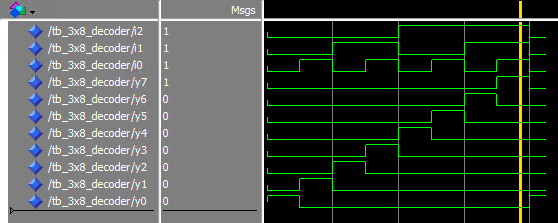
\includegraphics[width=\textwidth]{./diagrams/3x8_simulation.png}
\end{figure}
%-------------------- 3x8 decoder END --------------------
\clearpage
%-------------------- 8x3 p-encoder begin --------------------
\section{Exercise D: 8-to-3 Priority Encoder}
\subsection{Objective}
The purpose of this exercise was to create a 8x3 priority encoder circuit from its respective combinational logic. Now having compiled and generated the relevant VHDL for the circuit one was able to simulate the circuit in action. Thus resulting in a better understanding of designing a 8x3 priority encoder circuit from its respective combinational equation, and testing that created circuit.

\subsection{Functionality and Specifications}
\[
\begin{aligned}
Y_2 &= D_7 + D_6 + D_5 + D_4,\\[1mm]
Y_1 &= D_7 + D_6 + \overline{D_7 + D_6}\,(D_3 + D_2),\\[1mm]
Y_0 &= D_7 + \overline{D_7 + D_6}\,D_5 + \overline{D_7 + D_6 + D_5}\,D_3 + \overline{D_7 + D_6 + D_5 + D_4}\,D_1.
\end{aligned}
\]

Here we want to describe the combinational logic functions (our equations essentially )

\begin{figure}[h]
\caption{8x3 priority encoder}
\centering
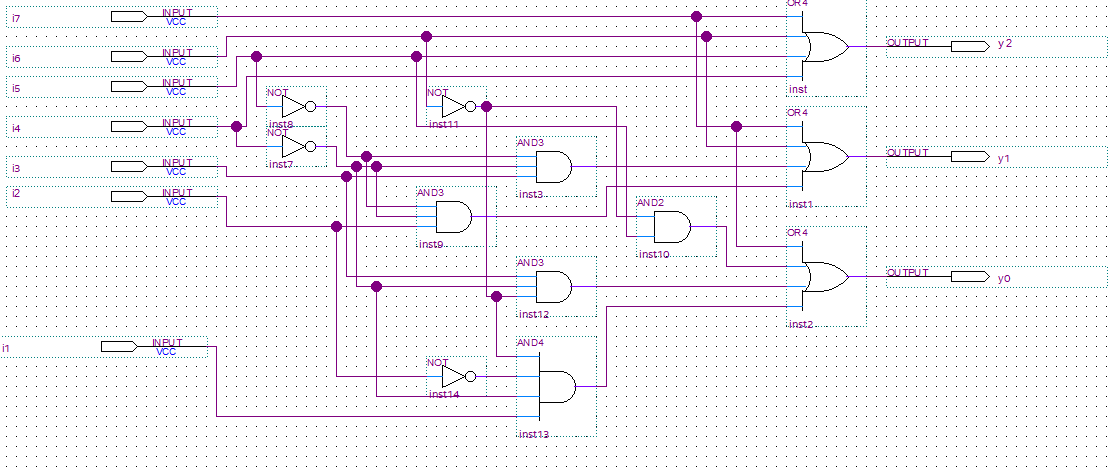
\includegraphics[width=\textwidth]{./diagrams/8x3_penc_design.png}
\end{figure}
{VHDL code generated from design file}
\begin{minted}{vhdl}
    LIBRARY ieee;
    USE ieee.std_logic_1164.all;

    LIBRARY work;

    ENTITY \8x3_p_enc\ IS
    	PORT
    	(
    		i2 :  IN  STD_LOGIC;
    		i1 :  IN  STD_LOGIC;
    		i3 :  IN  STD_LOGIC;
    		i4 :  IN  STD_LOGIC;
    		i5 :  IN  STD_LOGIC;
    		i6 :  IN  STD_LOGIC;
    		i7 :  IN  STD_LOGIC;
    		y2 :  OUT  STD_LOGIC;
    		y1 :  OUT  STD_LOGIC;
    		y0 :  OUT  STD_LOGIC
    	);
    END \8x3_p_enc\;

    ARCHITECTURE bdf_type OF \8x3_p_enc\ IS

    SIGNAL	SYNTHESIZED_WIRE_0 :  STD_LOGIC;
    SIGNAL	SYNTHESIZED_WIRE_1 :  STD_LOGIC;
    SIGNAL	SYNTHESIZED_WIRE_15 :  STD_LOGIC;
    SIGNAL	SYNTHESIZED_WIRE_16 :  STD_LOGIC;
    SIGNAL	SYNTHESIZED_WIRE_6 :  STD_LOGIC;
    SIGNAL	SYNTHESIZED_WIRE_8 :  STD_LOGIC;
    SIGNAL	SYNTHESIZED_WIRE_9 :  STD_LOGIC;
    SIGNAL	SYNTHESIZED_WIRE_10 :  STD_LOGIC;
    SIGNAL	SYNTHESIZED_WIRE_17 :  STD_LOGIC;


    BEGIN



    y2 <= i7 OR i5 OR i4 OR i6;


    y1 <= i7 OR SYNTHESIZED_WIRE_0 OR SYNTHESIZED_WIRE_1 OR i6;


    SYNTHESIZED_WIRE_10 <= SYNTHESIZED_WIRE_15 AND i5;


    SYNTHESIZED_WIRE_15 <= NOT(i6);



    SYNTHESIZED_WIRE_8 <= i3 AND SYNTHESIZED_WIRE_16 AND SYNTHESIZED_WIRE_15;


    SYNTHESIZED_WIRE_9 <= SYNTHESIZED_WIRE_15 AND SYNTHESIZED_WIRE_6 AND SYNTHESIZED_WIRE_16 AND i1;


    SYNTHESIZED_WIRE_6 <= NOT(i2);



    y0 <= i7 OR SYNTHESIZED_WIRE_8 OR SYNTHESIZED_WIRE_9 OR SYNTHESIZED_WIRE_10;


    SYNTHESIZED_WIRE_0 <= SYNTHESIZED_WIRE_17 AND SYNTHESIZED_WIRE_16 AND i3;


    SYNTHESIZED_WIRE_16 <= NOT(i4);



    SYNTHESIZED_WIRE_17 <= NOT(i5);



    SYNTHESIZED_WIRE_1 <= SYNTHESIZED_WIRE_17 AND SYNTHESIZED_WIRE_16 AND i2;


    END bdf_type;

\end{minted}

\subsubsection{VHDL code for Test bench}
\begin{minted}{vhdl}
    library IEEE;
    use IEEE.STD_LOGIC_1164.ALL;
    use IEEE.STD_LOGIC_TEXTIO.ALL;
    use std.textio.all;

    entity tb_8x3_p_encoder is
    end tb_8x3_p_encoder;

    architecture test of tb_8x3_p_encoder is
        signal i1 : STD_LOGIC;
        signal i2 : STD_LOGIC;
        signal i3 : STD_LOGIC;
        signal i4 : STD_LOGIC;
        signal i5 : STD_LOGIC;
        signal i6 : STD_LOGIC;
        signal i7 : STD_LOGIC;
        signal y2 : STD_LOGIC;
        signal y1 : STD_LOGIC;
        signal y0 : STD_LOGIC;

        component \8x3_p_enc\
            Port ( i1 : in STD_LOGIC;
                   i2 : in STD_LOGIC;
                   i3 : in STD_LOGIC;
                   i4 : in STD_LOGIC;
                   i5 : in STD_LOGIC;
                   i6 : in STD_LOGIC;
                   i7 : in STD_LOGIC;
                   y2 : out STD_LOGIC;
                   y1 : out STD_LOGIC;
    	       y0 : out STD_LOGIC);
        end component;

    begin
        uut: \8x3_p_enc\ port map(i1, i2, i3, i4, i5, i6, i7, y2, y1, y0);
        PROCESS
        BEGIN
    	-- No inputs active
            i1 <= '0';
            i2 <= '0';
            i3 <= '0';
            i4 <= '0';
            i5 <= '0';
            i6 <= '0';
            i7 <= '0';
            WAIT for 20 ns;
            -- i1 active
            i1 <= '1';
            i2 <= '0';
            i3 <= '0';
            i4 <= '0';
            i5 <= '0';
            i6 <= '0';
            i7 <= '0';
            WAIT for 20 ns;
            -- i2 active
            i1 <= '0';
            i2 <= '1';
            i3 <= '0';
            i4 <= '0';
            i5 <= '0';
            i6 <= '0';
            i7 <= '0';
            WAIT for 20 ns;
            -- i3 active
            i1 <= '0';
            i2 <= '0';
            i3 <= '1';
            i4 <= '0';
            i5 <= '0';
            i6 <= '0';
            i7 <= '0';
            WAIT for 20 ns;
            -- i4 active
            i1 <= '0';
            i2 <= '0';
            i3 <= '0';
            i4 <= '1';
            i5 <= '0';
            i6 <= '0';
            i7 <= '0';
            WAIT for 20 ns;
            -- i5 active
            i1 <= '0';
            i2 <= '0';
            i3 <= '0';
            i4 <= '0';
            i5 <= '1';
            i6 <= '0';
            i7 <= '0';
            WAIT for 20 ns;
            -- i6 active
            i1 <= '0';
            i2 <= '0';
            i3 <= '0';
            i4 <= '0';
            i5 <= '0';
            i6 <= '1';
            i7 <= '0';
            WAIT for 20 ns;
            -- i7 active
            i1 <= '0';
            i2 <= '0';
            i3 <= '0';
            i4 <= '0';
            i5 <= '0';
            i6 <= '0';
            i7 <= '1';
            WAIT for 20 ns;
            -- multiple active, output should be: (Highest priority, i7)
            i1 <= '0';
            i2 <= '0';
            i3 <= '1';
            i4 <= '0';
            i5 <= '1';
            i6 <= '0';
            i7 <= '1';
            WAIT for 20 ns;
            -- multiple active, output should be: (Highest priority, i6)
            i1 <= '1';
            i2 <= '1';
            i3 <= '1';
            i4 <= '1';
            i5 <= '0';
            i6 <= '1';
            i7 <= '0';
            WAIT for 20 ns;
            -- multiple active, output should be: (Highest priority, i5)
            i1 <= '1';
            i2 <= '1';
            i3 <= '1';
            i4 <= '1';
            i5 <= '1';
            i6 <= '0';
            i7 <= '0';
            WAIT for 20 ns;
            -- multiple active, output should be: (Highest priority, i4)
            i1 <= '1';
            i2 <= '1';
            i3 <= '1';
            i4 <= '1';
            i5 <= '0';
            i6 <= '0';
            i7 <= '0';
            WAIT for 20 ns;
            -- multiple active, output should be: (Highest priority, i3)
            i1 <= '1';
            i2 <= '1';
            i3 <= '1';
            i4 <= '0';
            i5 <= '0';
            i6 <= '0';
            i7 <= '0';
            WAIT for 20 ns;
            -- multiple active, output should be: (Highest priority, i2)
            i1 <= '1';
            i2 <= '1';
            i3 <= '0';
            i4 <= '0';
            i5 <= '0';
            i6 <= '0';
            i7 <= '0';
            WAIT for 20 ns;

        END PROCESS;

    end test;

\end{minted}


\subsection{Simulation}
In this simulation part regarding the (Draw truth tables based on the waveforms.) part we just compare the wave form against the
\begin{figure}[h]
\caption{8x3 priority encoder wave graph}
\centering
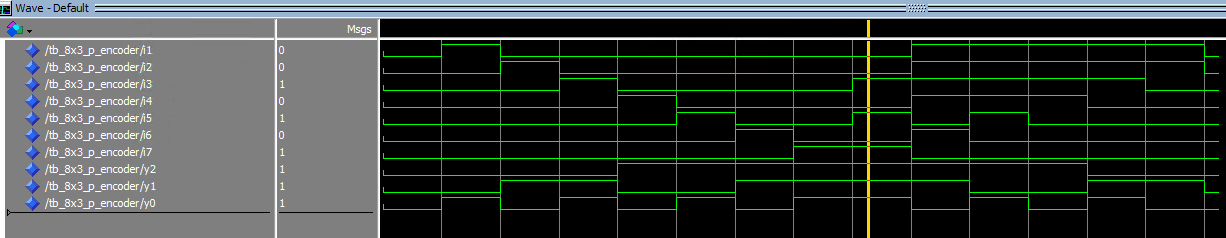
\includegraphics[width=\textwidth]{./diagrams/8x3_p_enc_simulation.png}
\end{figure}

%-------------------- 8x3 p-encoder END --------------------
\clearpage
%-------------------- SR latch & Flip flop begin --------------------
\section{Exercise E: Set-Reset Flip-Flop \& D Flip-Flop (Positive Edge Trigger)}
\subsection{Objective}

\subsection{Functionality and Specifications}

\subsection{Simulation}
%-------------------- SR latch & Flip flop END --------------------

\section{Conclusions}

\end{document}